%\documentclass[a4paper,11pt]{article}
\documentclass[a4paper,11pt]{scrartcl}

\usepackage[utf8]{inputenc}
\usepackage[italian]{babel}

\usepackage{graphicx} %for includng images
\graphicspath{{img/}}

\usepackage{siunitx} % package for deciBel and other units

\usepackage{amsmath} % package for ``cases'' and other matemagical stuff

\usepackage[american]{circuitikz} % circuit drawer
\ctikzset{/tikz/circuitikz/bipoles/length=1cm} %dimensione componenti

\usepackage{subcaption}  %per immagini multiple

%\usepackage{xcolor} % Colori!
\usepackage{colortbl} %colori nelle tabelle!!

\usepackage{multirow} %righe doppie nelle tabelle

\usepackage{makecell} %multirow box

\title{Appunti di Principi di Ingegneria Elettrica II}
\author{Daniele Olivieri}
\date{}

\pdfinfo{%
  /Title    ()
  /Author   ()
  /Creator  ()
  /Producer ()
  /Subject  ()
  /Keywords ()
}
%\includeonly{}
\begin{document}
\maketitle
\setlength\arrayrulewidth{1.2pt} %larghezza righe tabelle
\section{Introduzione ai circuiti dinamici}
Tutti i circuiti che contengono componenti come
resistori, induttori e condensatori, generatori indipendenti di tensione e corrente ai quali si associa 
una tensione impressa o una corrente impressa vengono detti circuiti lineari tempo invarianti (LTI).

Se vi sono anche bipoli tempo-varianti come interruttori che si chiudono o si aprono, il circuito
si definisce lineare tempo variante (LTV).

Preso un generico circuito, si vuole determinare una tensione o un'intensità di corrente di un generico
bipolo.

\textbf{Strumenti a disposizione:}

\begin{itemize}
\item Equazioni di interconnessione:
\begin{equation} \label{eq:leggi_kirchooff}
\begin{cases}
        \text{LKC} & \forall \text{ nodo } \sum_{k} (\pm) i_k(t) = 0\ \forall\ t \\
        \text{LKT} & \forall \text{ maglia } \sum_{h} (\pm) v_n(t) = 0\ \forall\ t
\end{cases}
\end{equation}

\item Relazioni caratteristiche dei bipoli coerenti con la scelta dei versi delle grandezze (convenzione del generatore o dell'utilizzatore).
\begin{equation}
\begin{cases}
v_R  = R\cdot i \\
v_L  = L\frac{di_L}{dt} \\
i_C  = C\frac{dv_C}{dt} \\
v_e  = e(t)\\
i_j  = j(t) \\
\end{cases}
\end{equation}
\begin{equation*}
\begin{cases}
\text{interruttori in chiusura a t=0: }  {t<0,\ i = 0\ \forall\ v;\ t > 0,\ v = 0\ \forall\ i} \\
\text{interruttori in apertura a t=0: }  {t<0,\ v = 0\ \forall\ i;\ t > 0,\ i = 0\ \forall\ v} 
\end{cases}
\end{equation*}
\end{itemize}

Le equazioni di interconnessione non sono tutte indipendenti ma è sempre possibile
costruire un set di equazioni indipendenti scegliendo \textit{n-1} nodi o \textit{n-l-1} maglie fondamentali,
dove n ed l sono rispettivamente il numero di nodi e lati del grafo connesso.

NOTA: per ogni induttore la potenza assorbita:
$$ P^a(t) = v_l\cdot i_l = L \frac{di_L}{dt}\cdot i_l = \frac{d}{dt} \left[\frac{1}{2}Li_L^2\right] = \frac{dW_m}{dt} $$ 
L' energia immagazzinata nel campo magnetico dell'induttore invece:
$$\Delta W^a(t_1,t_2) = \int_{t_1}^{t_2} P^a(\tau)d\tau = W_m (t_2) - W_m(t_1) $$
Se in un certo istante di tempo l'induttore presenta una certa quantità di energia in Joule [\si{\joule}] quella sarà la massima energia estraibile.

Per ogni condensatore invece potenza ed energia sono così definite:
$$P^a(t) = \frac{d}{dt} W_e;\ W_e(t) = \frac{1}{2} CV_c^2$$
L'energia sarà immagazzinata mediante il campo elettrico.

Si ha quindi un sistema di equazioni circuitali in cui si ha una parte algebrica con le caratteristiche adinamiche, ossia con caratteristiche
non differenziali e non integrali, più una parte differenziale data dai bipoli dinamici come condensatori e induttori.
In letteratura un sistema simile si indica con DAE (Differential Algebric Equation), differente
dalla ODE (Ordinary Differential Equation).

Le tecniche utilizzate in teoria dei circuiti mirano a trasformare una DAE in una ODE, ossia 
formulare le equazioni circuitali come equazioni differenziali ordinarie, per operare questa trasformazione si fa 
riferimento alla dinamica delle sole {variabili di stato}: $i_l(t),\ v_c(t)$

La loro conoscenza permette di esprimere tutte le altre variabili attraverso relazioni algebriche, vengono definite
variabili \textit{slaved}, perché subordinate alle prime.

Per eseguire ciò si richiama una procedura generale per l'analisi di circuiti lineari tempo varianti (LTV).
Questa procedura si basa su un'analisi a intervallo: si partiziona l'asse dei tempi in intervalli in ciascuno dei 
quali esiste un circuito tempo invariante (LTI) equivalente a quello di partenza.

\begin{figure}[H] %tre stati diversi dello stesso circuito
\centering
 \begin{subfigure}{.3\textwidth}
  \centering
  \caption{configurazione generica}
  \begin{circuitikz}
   \draw (0,0) to [R] (1,0);
   \draw (0,0.6) to [L] (1,0.6);
   \draw (0,1.2) to [C] (1,1.2);
   \draw (0,1.8) to [V] (1,1.8);
   \draw (0,2.4) to [I] (1,2.4);
   \draw (0,3) to [closing switch] (1,3);
   \draw (0,3.6) to [opening switch] (1,3.6);
   \draw (-0.3,-0.3) rectangle (1.3,3.9);
  \end{circuitikz}
 \end{subfigure}
 \begin{subfigure}{.3\textwidth}
  \centering
  \caption{$t<0$}
  \begin{circuitikz}
   \draw (0,0) to [R] (1,0);
   \draw (0,0.6) to [L] (1,0.6);
   \draw (0,1.2) to [C] (1,1.2);
   \draw (0,1.8) to [V] (1,1.8);
   \draw (0,2.4) to [I] (1,2.4);
   \draw (0,3) to [open,o-o] (1,3);
   \draw (0,3.6) to [short] (1,3.6);
   \draw (-0.3,-0.3) rectangle (1.3,3.9);
  \end{circuitikz}
 \end{subfigure}
 \begin{subfigure}{.3\textwidth}
  \centering
  \caption{$t>0$}
  \begin{circuitikz}
   \draw (0,0) to [R] (1,0);
   \draw (0,0.6) to [L] (1,0.6);
   \draw (0,1.2) to [C] (1,1.2);
   \draw (0,1.8) to [V] (1,1.8);
   \draw (0,2.4) to [I] (1,2.4);
   \draw (0,3) to [short] (1,3);
   \draw (0,3.6) to [open,o-o] (1,3.6);
   \draw (-0.3,-0.3) rectangle (1.3,3.9);   
  \end{circuitikz}
 \end{subfigure}
\end{figure}

Supponendo che i generatori indipendenti abbiano grandezze \textbf{limitate}, ossia le tensioni impresse $e(t)$ e le correnti impresse $j(t)$,
in questa ipotesi si sa che le variabili di stato sono funzioni \textbf{continue} ossia:
\begin{equation*}
\begin{split}
i_L (0^+) & = i_L(0^-) \\
v_C (0^+) & = v_C(0^-)
\end{split}
\end{equation*}

La soluzione si determina trovando la dinamica delle variabili di stato in ciascun circuito ausiliario, "incollando" le soluzioni utilizzando la proprietà di continuità delle variabili di stato.

Il problema di risolvere circuiti lineari tempo varianti si scompone nel risolvere tanti circuiti lineari tempo invarianti. Una categoria semplice di circuiti tempo invarianti sono i
circuiti lineari del primo ordine (circuiti RC o RL) con un solo elemento dinamico.
\begin{figure}[H] %circuiti RC ed RL equivalenti
\centering
 \begin{subfigure}{.3\textwidth}
  \centering
  \begin{circuitikz}
   \draw (0,0) rectangle (1.6,1.7);
   \draw (0.3,0.3) to [I] (1.3,0.3);
   \draw (0.3,0.9) to [V] (1.3,0.9);
   \draw (0.3,1.5) to [R] (1.3,1.5);
   \draw (1.6,1.5) to [short,i=$i_C$] (2,1.5)
   to [C,v^=$v_C $] (2,0.4) to [short] (1.6,0.4);
  \end{circuitikz}
  \caption{Circuito RC}
 \end{subfigure} 
  \begin{subfigure}{.3\textwidth}
  \centering
  \begin{circuitikz}
   \draw (0,0) rectangle (1.6,1.7);
   \draw (0.3,0.3) to [I] (1.3,0.3);
   \draw (0.3,0.9) to [V] (1.3,0.9);
   \draw (0.3,1.5) to [R] (1.3,1.5);
   \draw (1.6,1.5) to [short,i=$i_L $] (2,1.5)
   to [L,v^=$v_L $] (2,0.4) to [short] (1.6,0.4);
  \end{circuitikz}
  \caption{circuito RL}
 \end{subfigure}
\end{figure}

Un bipolo adinamico lineare e un bipolo dinamico fanno subito pensare all'utilizzo dei teoremi di Thévenin e Norton, permettendo la riduzione del circuito 
adinamico ad un semplice generatore con un resistore equivalente.

Applicando ad esempio la LKT $e_0(t) = R_{th}\cdot C \frac{dV_C}{dt} + V_C$ si ha l'equazione di stato
del circuito e supponendo di conoscere $V_C(t=0) = V_0 $ allora la soluzione dell'equazione è:
$$V_C(t) = [V_0-V_{C_p}(0)] e^{-\frac{t}{\tau}} + V_{C_p}(t)$$ dove $\tau = R_{th}\cdot C$ e $V_{C_p}(t)$
è la soluzione a regime. 
 
Dopo un intervallo pari a $4\sim 5\ \tau$ si assume il processo di carica o scarica terminato.

Per il circuito RL 
$$I_L(t) = [I_0-I_{L_p}(0)]e^{-\frac{t}{\tau}} + I_{L_p}(t)$$ 
con $\tau = \frac{L}{R_{th}},\ I_0 = I_L (t=0)$

Osservazione: la soluzione generale del circuito RC, ossia la dinamica di $V_c(t)$ può essere espressa 
come la somma di due termini $V_{C_{tr}}(t)$ e $V_{C_p}(t)$, il primo transitorio, che tende a svanire se 
si attende un tempo sufficiente lungo, porta con se la \textit{memoria} dello stato iniziale, memoria che 
viene
persa quando $t>4\sim5\ \tau$, ammesso che $\tau$ sia positiva; esistono infatti alcune combinazioni di 
elementi circuitali che si comportano come un resistore negativo.

Il secondo termine è quello di regime permanente, che ovviamente non ha memoria dello stato iniziale ma 
dipende solo dalla nuova configurazione
del circuito (termine forzato).

La decomposizione in regime transitorio e permanente è una decomposizione generale che vale per qualsiasi circuito, a patto di complicare opportunamente la matematica.

Si parla quindi di evoluzione libera ed evoluzione forzata 
$$\begin{cases}
e_0(t) = R_{th}C\frac{dV_c}{dt} + V_C \\
V_c(0) = V_0
\end{cases}$$
si scompone in:

Evoluzione libera
$$\begin{cases}
0 &= R_{th}C\frac{dV_c}{dt} + V_C \\ 
V_c(0) &= V_0
\end{cases}$$

Evoluzione forzata
$$\begin{cases}
e_0(t) &= R_{th}C\frac{dV_c}{dt} + V_C \\
V_c(0) &= 0
\end{cases}$$

Trattazione analoga (duale) per il circuito RL

\newpage
\subsection{Circuiti lineari tempo invarianti del II ordine}
Divisi in (RC, RL, RLC), la procedura generale di risoluzione richiede tre step:
\begin{enumerate}
 \item Determinazione delle equazioni di stato
 \item Determinazione delle condizioni iniziali
 \item Soluzione del problema di Cauchy
\end{enumerate}

Esempio:
\begin{figure}[H]
\centering
\begin{circuitikz}
 \draw (0,2) to [V,l_=$E$] (0,0);
 \draw (0,2) to [closing switch=${t=0}$](1,2) 
             to [R,l=$R_1$] (2.5,2)
             to [R,l=$R_2$] (4,2)
             to [L,i=$i_L$,l=$L$] (4,0)
             to [short] (0,0);
 \draw (2.5,2)node[circ,color=red]{} to [C,v=$v_C$,l=$C$] (2.5,0);
\end{circuitikz}
\caption{Esempio di un circuito RLC del secondo ordine}
\end{figure}

La dinamica dello stato per $t<0$ è di facile risoluzione, $i_L(t) = 0$, $v_C(t) = 0$
per $t > 0$ invece si analizza il circuito:

Equazioni di interconnessione: 
LKC nel nodo evidenziato in rosso (tra i due resistori)
\begin{equation*}
\begin{cases}
I_1 &= I_C+i_L \ \qquad \text{LKC}\\
E &= R_1\cdot I_1 + v_C\ \qquad \text{LKT} \\
v_C &= R_2 \cdot i_L + V_L\ \qquad \text{LKT} \\
V_L &= L\frac{di_L}{dt} \\
I_C &= C\frac{dv_C}{dt}
\end{cases}
\end{equation*}
Si ricava $I_1$ dalla seconda e si sostituisce nella prima,
ora si ricavano le variabili di stato ottenendo
$$
\begin{cases}
i_C = \frac{E}{R_2} - \frac{v_C}{R_1} - i_L \\
v_L = v_C - R_2 i_L
\end{cases}
$$
Sostituendo le equazioni caratteristiche dei bipoli dinamici:

$$
\begin{cases}
C\frac{dv_C}{dt} = \frac{E}{R_2} - \frac{v_C}{R_1} - i_L \\
L\frac{di_L}{dt} = v_C - R_2 i_L
\end{cases}
$$

Le condizioni iniziali sono 
$$\begin{cases}
v_C(0^+) = v_C(0^-) = 0\\
i_L(0^+) = i_L(0^-) = 0
\end{cases}
$$
Per risolvere queste equazioni conviene ridurle ad un'equazione del secondo ordine ad una sola incognita,
ad esempio si sostituisce nell'equazione che definisce $i_C$, $v_C$ ricavata dalla equazione di
$v_L$, in questo modo si ha un'unica equazione in cui compaiono le grandezze relative all'induttore.

Si ottiene 
\begin{equation}
LC \frac{d^2i_L}{dt^2} + CR_2\frac{di_L}{dt} = \frac{E}{R_1} - \frac{L}{R_1}\frac{di_L}{dt} - \frac{R_2}{R_1}i_L-i_L
\end{equation}
raccogliendo i termini
$$
\frac{d^2i_L}{dt^2} + \left(\frac{R_2}{L} + \frac{1}{R_1C}\right)\frac{di_L}{dt}+ \left(1 + \frac{R_2}{R_1}\right)\frac{1}{LC} i_L = \frac{E}{R_1}\frac{1}{LC}
$$
%ora raccogli i termini
Controlli da eseguire: controllo dimensionale e positività dei coefficienti altrimenti il circuito non sarebbe dissipativo.

L'integrale generale è scritto come somma dell'integrale dell'omogenea associata e dell'integrale particolare.
Si ottiene il polinomio caratteristico a partire dall'omogenea associata, ossia annullando il forzamento:
\begin{equation}
\lambda^2 + \left(\frac{R_2}{L} + \frac{1}{R_1 C}\right)\lambda + \left(1+\frac{R_2}{R_1}\right)\frac{1}{LC} = 0
\end{equation}
La soluzione del polinomio può essere di tre tipi:

\begin{itemize}
\item Caso 1, radici reali e distinte, solitamente negative in sistemi dissipativi, modi naturali aperiodici 
smorzati
$$
i_{L_0} = K_1 e^{\lambda_1 t} + K_2 e^{\lambda_2 t}
$$
\begin{figure}[H]
\centering
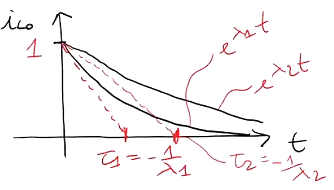
\includegraphics[width=0.4\linewidth]{evoluzione_libera_reali_distinte}
\end{figure}


\item Caso 2, radici reali e coincidenti, caso piuttosto patologico
la radice viene determinata con $-\sigma$ si avrà un modo esponenziale decrescente $e^{-\sigma t} $ con
$\tau = \frac{1}{\sigma}$ e un modo pari a  $t\cdot e^{-\sigma t}$
$$
i_{L_0} = K_1 e^{-\sigma t} + K_2 t\cdot e^{-\sigma t}
$$
\begin{figure}[H]
\centering
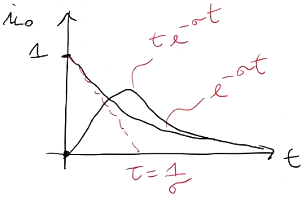
\includegraphics[width = 0.4\linewidth]{evoluzione_libera_reali_coincidenti}
\end{figure}
Vengono detti modi aperiodici smorzati con smorzamento critico.


\item Caso 3, modi periodici smorzati, soluzioni complesse coniugate
$\lambda_{1,2} = -\sigma \pm j\omega_d$, la distanza tra due picchi è pari a $\frac{2\pi}{\omega_d}$
$$i_{L_0}(t) = e^{-\sigma t} [K_1 \cos (\omega_d t) + K_2 \sin(\omega_d t)]$$
\begin{figure}[H]
\centering
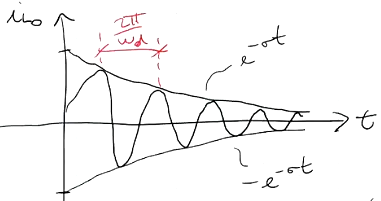
\includegraphics[width=0.4\linewidth]{evoluzione_libera_complesse_coniugate}
\end{figure}
\end{itemize}

Restano da determinare le costanti di integrazione imponendo le condizioni iniziali,
\begin{equation*}
\begin{cases}
i_L(0^+) = i_L(0^-) = \SI{0}{\ampere}\\
\frac{di_L}{dt}(0^+) = \frac{1}{L}[v_C(0^+) - R_2i_L(0^+)] = 0
\end{cases}
\end{equation*}

Supponendo dunque di avere soluzioni $\lambda_1,\ \lambda_2$ reali e distinte e ricordando di aggiungere
il termine a regime $\frac{E}{R_1 + R_2}$ nella determinazione dei coefficienti
$$
\begin{aligned}
i_L(0^+) = 0 & \Rightarrow \\
\frac{di_L}{dt}(0^+) = 0 & \Rightarrow
\end{aligned}
\begin{cases}
K_1+K_2 + \frac{E}{R_1+R_2} = 0 \\
\lambda_1K_1 + \lambda_2K_2 = 0
\end{cases}
$$
La soluzione del sistema permette di ricavare i coefficienti $K_1$ e $K_2$

%Lezione 2 i minuti si riferiranno a quelli visibili su teams e non quelli del file registrato con OBS
\section{Determinazione equazioni di stato di un circuito qualsiasi}

Si riprende la classe di circuiti lineari tempo invarianti (LTI), supponiamo di conoscere
le variabili di stato $i_L(t) $ e $v_C(t) $ assumendole note, sostituiamo ogni \textit{condensatore}
con un generatore di tensione di valore pari alla $v_C(t)$ , ripetendo il procedimento
per ciascun \textit{induttore} che viene sostituito con un generatore di corrente con corrente impressa
pari a $i_L(t)$.

In queste condizioni, la soluzione del circuito resta formalmente invariata.
Il nuovo circuito sarà di tipo adinamico, non presenterà più alcun componente dinamico, il nuovo circuito
prende il nome di \textit{circuito resistivo associato al circuito di partenza}.

Il vantaggio di questa operazione è la possibilità di ricavare $v_L$ e $i_C$ utilizzando il principio
di \textit{sovrapposizione degli effetti} (PSE).

Si ricavano le equazioni di stato per il seguente circuito:
26:07

\begin{figure}[h]

\end{figure}

Si applica il PSE, per trovare $i_C$ e $v_L$:
$$
i_C = i_c' + i_C'' + i_C '''
$$
$$
v_L = v_L' + v_L'' + v_L'''
$$

Disegna circuiti 28:48

Circuito 1)
$$
v_L' = 0;\ i_C' = \frac{E}{R_1} 
$$
Circuito 2)
$$
i_C'' = -\frac{v_C}{R_1};\ v_L'' = v_C
$$
Circuito 3)
$$
i_C''' = -i_L;\ v_L''' = -R_2\cdot i_L
$$

Sommando i tre contributi:
$$
i_C = \frac{E}{R_1} - \frac{v_C}{R_1} - i_L = C\frac{dv_C}{dt}
$$
$$
v_L = v_C - R_2\cdot i_L = L\frac{di_L}{dt}
$$
con le condizioni di continuità delle variabili di stato:
$$
i_L(0^+) = i_L(0^-)
$$
$$
v_C(0^+) = v_C(0^-)
$$

\section{Circuiti lineari con generazioni impulsivi}
Si analizza ora un circuito che presenta generatori di tipo impulsivo, ad esempio la risposta di 
una linea elettrica a seguito di una fulminazione.
Si definisce quindi l'impulso rettangolare di ammpiezza $\Delta$, la funzione viene chiamata 
$\Pi_\Delta(t)$,(funzione porta) è costante nell'intervallo $[-\frac{\Delta}{2},\frac{\Delta}{2}]$,
l'area del rettangoloide sotteso alla funzione è pari a
$$
\int_{-\Delta/2}^{\Delta/2}\Pi_\Delta(\tau)d\tau = 1\ \forall\ \Delta \in\ ]0,+\infty[
$$
Ha senso considerare la successione di funzioni ottenute per valori $\Delta$ decrescenti,
ma dimezzando la base, per mantenere l'area unitaria, va raddoppiata l'altezza.

Passando al limite per $\Delta \rightarrow 0^+$ la successione tende in maniera non ordinaria
ad un limite che non è una funzione ma può essere definita come funzione generalizzata,
ossia distribuzione, che prende il nome di \textbf{Delta di Dirac} ($\delta(t)$).

Proprietà della delta:
\begin{itemize}
\item È nulla $\forall t \neq 0$
\item Ha integrale unitario
\item Proprietà di campionamento $\int_{-\infty}^{+\infty}f(\tau)\delta(\tau-t_0)d\tau = f(t_0)$
\end{itemize}
Esempio della proprietà di campionamento: 49:03
$$
\int_{-\Delta/2}^{\Delta/2} f(\tau)\Pi_\delta(\tau-t_0)d\tau = \frac{1}{\Delta} \int_{-\Delta/2}^{\Delta/2}  f(\tau)d\tau = f(\vartheta^*)
$$


Analizziamo un'altra funzione $U_\Delta(t)$ definita come segue:
\begin{equation*}
\begin{cases}
0\ ,& t  < -\frac{\Delta}{2} \\
1\ ,& t  > \frac{\Delta}{2} \\
\frac{1}{2}+\frac{t}{\Delta}\ ,& -\frac{\Delta}{2} \leq t \leq \frac{\delta}{2}
\end{cases}
\end{equation*}
Rampa 55:03

Eseguendo la derivata temporale si otterrà la funzione $\Pi_\Delta(t)$, al limite di $\Delta \rightarrow 0$
si ottiene la funzione definita ``gradino'' o funzione di Heaviside $u(t)$.

Un ulteriore modo per definire la $\delta(t)$ è appunto quella di derivata della funzione gradino $u(t)$.
$$
\delta(t) = \frac{d}{dt}u(t) \Leftrightarrow \int_{-\infty}^t \delta(\tau)d\tau = u(t)
$$

\paragraph{Esempio con generatore impulsivo}
Si prenda un circuito RC serie 01:12:00 e una funzione $e(t)$ che vale $E_0$ per $0 < t < T$ e $0$ 
altrimenti.
Ricaviamo $v_C(t)$:

Si suppone che la condizione iniziale, ossia per $t < 0 $, la tensione sul condensatore sia nulla.

\begin{equation*}
\begin{cases}
e(t) &= RC\frac{dv_C}{dt} + v_C \\
v_C(0) &= 0
\end{cases}
\end{equation*}

$$
\begin{cases}
E_0 &= RC\frac{dv_C}{dt} + v_C \\
v_C^{(1)}(0) &= 0 \\
0 \leq t \leq T
\end{cases}
$$

$$
\begin{cases}
0 &= RC\frac{dv_C}{dt} + v_C \\
v_C^{(2)}(0) &= v_C^{(1)}(T) \\
t \geq T
\end{cases}
$$
Rivedi 1:19:00

Si ottiene una funzione esponenziale crescente fino a $T$ e poi decrescente fino a 0 all'infinito.
Diminuendo il valore di $T$ si vede che il ``picco'' della funzione sarà più basso, al limite 
di $T \rightarrow 0$ la soluzione si annulla.
Se imponiamo il prodotto $E_0\cdot T = 1$ ed eseguiamo il limite invece:
$$
\lim_{T\rightarrow0^+} v_C(t)
$$
Supponiamo di sviluppare la funzione esponenziale con la sua serie di Taylor:
$$
e^x = 1 + x + \frac{x^2}{2!} + \frac{x^3}{3!} + ... \Rightarrow 1-e^{-\frac{t}{\tau}} \simeq \frac{t}{\tau} 
$$

$$
\begin{cases}
0\ & t\leq 0 \\
\frac{1}{T}\frac{t}{\tau}\  & 0 \leq t\leq T \\
\frac{1}{T}\frac{T}{\tau} e^{-\frac{t-T}{\tau}}\ & t\geq T
\end{cases}
$$
Per $T\rightarrow 0^+$
$$
\begin{cases}
0\ & t\leq 0\\
\frac{1}{\tau}e^{\frac{-t}{\tau}}\ & t \geq 0
\end{cases}
$$

Il primo tratto dell'equazione si approssima quindi ad un tratto lineare fino a T, arrivando ad 
un'altezza di $\frac{1}{\tau}$ vedi figura 1:32:00

Se 
$$\Pi_\Delta(t) \stackrel{\Delta\rightarrow0^+}{\rightarrow} \delta(t) \Rightarrow v_C(t) \rightarrow h(t)$$
$h(t)$ è chiamata risposta all'impulso del circuito dinamico.

$$
\delta(t) = RC\frac{dv_C}{dt} + v_C \Leftarrow i_C = \frac{\delta(t)-v_C}{R}
$$
Se la tensione è impulsiva anche la corrente nel condensatore sarà di tipo impulsivo
$$
i_c = C\frac{dv_C}{dt} \Rightarrow \int_{0^-}^{0^+} i_C(\tau)d\tau = e[v_C(0^+)-v_C(0^-)]
$$
$$
v_C(0^+) - v_C(0^-) = \frac{1}{RC} \int_{0^-}^{0^+} \delta(\tau)d\tau - \frac{1}{RC} \int_{0^-}^{0^+} v_C(\tau)d\tau = \frac{1}{RC} = \frac{1}{\tau} \Rightarrow 
$$
$$
\Rightarrow v_C(0^+) = \frac{1}{RC} = \frac{1}{\tau}
$$
Rivedi discorso potenza 1:44:00

\paragraph{Risposta al gradino unitario di un circuito dinamico LTI}
Stesso circuito del precedente, ma stavolta si utilizza come forzamento il gradino unitario di
Heaviside, la soluzione è più semplice della precedente:

$$
v_C(t) = 1-e^{-\frac{t}{\tau}}u(t)
$$
la chiamiamo $g(t)$ e affermiamo che sia la risposta al gradino, richiamiamo la relazione
tra la funzione $\Pi_\Delta(t)$ e $U_\Delta(t)$ si ha che:
$$
\Pi_\Delta(t) = \frac{U_\Delta\left(t+\frac{\Delta}{2}\right)-U_\Delta\left(t-\frac{\Delta}{2}\right)}{\Delta} = e(t)
$$
per $\Delta \rightarrow 0^+$ ottengo $h(t) = v_C(t)$.

Essendo il circuito tempo invariante, si può trovare la risposta alla funzione $\Pi_\Delta(t)$
come combinazione lineare delle risposte delle due $U_\Delta$ opportunamente traslate, ossia
la risposta al gradino traslata.
$$
\text{Risp} \Pi_\Delta(t) = \frac{\text{Risp}\left\{U_\Delta\left(t+\frac{\Delta}{2}\right)\right\} - 
\text{Risp}\left\{U_\Delta\left(t-\frac{\Delta}{2}\right)\right\}}{\Delta} = 
\frac{g\left(t+\frac{\Delta}{2}\right) - g\left(t-\frac{\Delta}{2}\right)}{\Delta}
$$
Tutto si trasforma nella funzione rapporto incrementale della funzione $g(t)$ ossia
$$
\lim_{\Delta\rightarrow0^+}\text{Risp}\left\{\Pi_\Delta(t)\right\} = h(t) = \frac{dg}{dt}
$$

$$
h(t) = \frac{dg}{dt} = 0,\ t < 0;\ \frac{1}{\tau}e^{-\frac{t}{\tau}},\ t\geq0 
$$
La risposta all'impulso è quindi la derivata della risposta al gradino.

Si consideri un circuito RC serie
\begin{figure}[H]\centering
\begin{circuitikz}
\draw
(0,0) to [voltage source,invert,l=$u(t)$] (0,2)
      to [R=$R$] (2,2)
      to [C,l_=$C$,v^=$v_C$] (2,0) -- (0,0)
;
\end{circuitikz}
\end{figure}
si suppone che la tensione imposta al generatore sia un gradino unitario $u(t)$,
l'equazione di stato sarà:
$$
\begin{cases}
u(t) = RC \frac{dv_C}{dt} + v_C \\
v_C(0^+) = 0
\end{cases}
\Rightarrow v_C(t) = \left.
\begin{cases}
0 & t<0 \\
1-e^{-\frac{t}{\tau}} & t\geq 0
\end{cases}\right] = g(t)
$$

Si considera la funzione $U_\Delta$
$$U_\Delta(t) = 
\begin{cases}
0 & t< -\frac{\Delta}{2}\\
\frac{1}{2} + \frac{t}{\Delta} & -\frac{\Delta}{2} < t < \frac{\Delta}{2} \\
1 & t > \frac{\Delta}{2}
\end{cases}
$$
se si esegue la differenza di due funzioni $U_\Delta$ traslate di $\pm\frac{\Delta}{2}$ si ottiene 
una porta trapezoidale
$$
f(t) = \frac{U_\Delta\left(t+\frac{\Delta}{2}\right) - U_\Delta\left(t-\frac{\Delta}{2}\right)}{\Delta}
$$
tende ad una $\delta(t)$ delta di Dirac per $\Delta \rightarrow 0$.
Semplicemente si può invece definire la porta come differenza di due gradini traslati, in questo modo
si elimina il problema dei segmenti obliqui.

La linearità del sistema e la tempo-invarianza delle grandezze dei bipoli implica che la
risposta ad una combinazione lineare di funzioni traslate nel tempo si ottiene come combinazione lineare 
delle risposte dei singoli termini traslati.
$$
\text{Risp}\left\{\Pi_\Delta(t)\right\} = \frac{\text{Risp}\left\{u\left(t+\frac{\Delta}{2}\right) \right\} -\text{Risp}\left\{ u\left(t-\frac{\Delta}{2}\right) \right\}}{\Delta} = \frac{g\left(t+\frac{\Delta}{2}\right)-
g\left(t-\frac{\Delta}{2}\right)}{\Delta}
$$
Eseguendo il limite per $\Delta\to 0^+ $ si vede che quello appena presentato è un rapporto incrementale e
quindi
$$
\lim_{\Delta\to0^+} \Rightarrow \text{Risp} \left\{\delta(t)\right\} =h(t) = \frac{dg}{dt}
$$
Ricordando le funzioni $h(t)$ e $g(t)$ si vede la relazione
$$
h(t) = \begin{cases}
0 & t<0\\
\frac{1}{\tau}e^{-\frac{t}{\tau}} & t\geq 0
\end{cases}\qquad
g(t) = \begin{cases}
0 & t<0\\
1 - e^{-\frac{t}{\tau}} & t\geq 0
\end{cases} \Rightarrow
\frac{dg}{dt} = h(t)
$$
è possibile studiare la risposta all'impulso sfruttando quella al gradino, che è una funzione limitata e 
più semplice da analizzare.

\paragraph{Circuiti RC ed RL semplici con generatori impulsivi}
Si considerino 2 circuiti modello: il circuito RC parallelo e il circuito RL serie.

\begin{figure}[H]\centering
\begin{subfigure}{.4\textwidth}\centering
\begin{circuitikz}
\draw
(0,0) to [current source,l=$j(t)$] (0,2)
      to (1,2) to [R=$R$,i>^=$i_R$] (1,0) to (0,0);
\draw
(1,2) to (2.5,2)  to [C,l_=$C$,v^=$v_C(t)$,i>_=$i_C$] (2.5,0) -- (1,0)
;
\end{circuitikz}
\subcaption{RC parallelo}
\end{subfigure}
\begin{subfigure}{.4\textwidth}\centering
\begin{circuitikz}
\draw
(0,0) to [voltage source,invert,l=$e(t)$] (0,2)
      to [R,l_=$R$] (2.5,2) to [L,l_=$L$,i_>=$i_L(t)$,v^=$v_L$] (2.5,0) -- (0,0)
;
\end{circuitikz}
\subcaption{RL serie}
\end{subfigure}
\end{figure}

Siano i generatori impulsivi: $j(t) = Q\delta(t)$ ed $e(t) = \Phi\delta(t)$.
$$
j(t) = \frac{v_C}{R} + i_C = Q\delta(t) = \frac{v_C}{R} + C\frac{dv_C}{dt}
$$
Si integra la funzione nell'istante in cui è centrata la $\delta(t)$ ossia:
$$
\int_{0^-}^{0^+} Q\delta(\tau)d\tau  = \cancel{\int_{0^-}^{0^+}\frac{v_C}{R}d\tau} + C[v_C(0^+)-\cancel{v_C(0^-)}]
\Leftrightarrow Q = Cv_C(0^+) \ \ [Q] = \si{\coulomb} \text{ (Coulomb)}
$$
$$
\left[\int_{0^-}^{0^+} Q\delta(\tau)d\tau\right] = \text{ Coulomb}
$$
Tirando la costante $C$ fuori dall'integrale, che ha la dimensione di Coulomb, l'integrale rimanente
deve essere adimensionale.
Ciò significa che la $\delta(t)$ ha la dimensione di \si{\per\second} per essere coerente con l'integrale
e restituire una quantità finita.

\subparagraph{Caso duale con circuito RL:}

$$
e(t) = R\cdot i_L + v_L
$$
$$
\Phi\delta(t) = R\cdot i_L + L\frac{di_L}{dt}
$$
$$
\Phi\int_{0^-}^{0^+} \delta(\tau)d\tau = L i_L(0^+)\ , \ i_L(0^-) = 0
$$

Anche in questo caso per avere la dimensione del flusso in \si{\weber} per $\Phi$ allora la $\delta(t)$ 
avrà le dimensioni di \si{\per\second}.
\newpage
\subsection{Procedura generale per la risoluzione di circuiti con generatori impulsivi}
Si ha un circuito dinamico semplice al quale è collegato un generatore impulsivo,
si determina il circuito resistivo associato, ossia vengono sostituiti i condensatori con 
generatori di tensione e gli induttori con generatori di corrente.

Si ottiene un circuito parziale in cui si spengono i generatori interni (anche quelli equivalenti ai bipoli dinamici) e si lascia agire solo il generatore impulsivo.

Un ulteriore circuito è ottenuto facendo l'esatto contrario e spegnendo quindi il generatore impulsivo.

\begin{figure}[H]\centering
\begin{subfigure}{0.45\linewidth}\centering
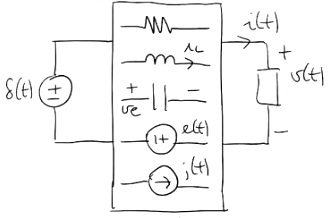
\includegraphics[width=\linewidth]{lezione_03_circuito_A}
\subcaption{Circuito iniziale}
\end{subfigure}
\begin{subfigure}{0.45\linewidth}\centering
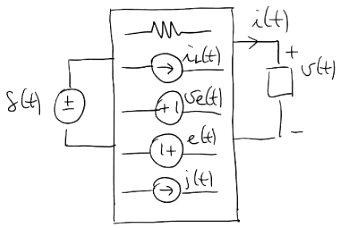
\includegraphics[width=\linewidth]{lezione_03_circuito_B}
\subcaption{Circuito resistivo associato}
\end{subfigure}
\begin{subfigure}{0.45\linewidth}\centering
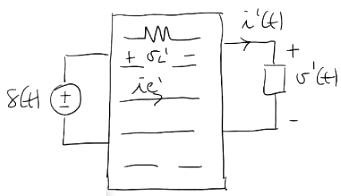
\includegraphics[width=\linewidth]{lezione_03_circuito_C-}
\subcaption{Circuito C'}
\end{subfigure}
\begin{subfigure}{0.4\linewidth}\centering
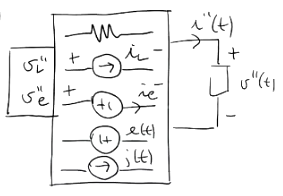
\includegraphics[width=\linewidth]{lezione_03_circuito_C--}
\subcaption{Circuito C"}
\end{subfigure}
\end{figure}
37:19
Si applica il PSE (Principio di Sovrapposizione degli effetti)
$$
\begin{cases}
v_L = v_L' + v_L''\\
i_C = i_C' + i_C''
\end{cases}
$$

Dal circuito C' si ricavano $v_L'$ e $i_C'$ causate dai generatori impulsivi 41:41

Viceversa dal circuito C'' si valutano le variabili di stato utilizzando come condizioni iniziali
le variabili ottenute in C'.

$$
v_C(0^+) = \frac{1}{C} \int_{0^-}^{0^+} i_C'(\tau)d\tau \ , \ v_C(0^-) = 0
$$
$$
i_L(0^+) = \frac{1}{L} \int_{0^-}^{0^+} i_L'(\tau)d\tau \ , \ i_L(0^-) = 0
$$
L'integrale delle variabili di stato del circuito C'' è pari a 0 dato che la funzione integranda è limitata
e l'intervallo è infinitesimo.

Infine si risolve il circuito C'' usando le variabili di stato appena calcolate in C'.

Esercizio 

Conclusione dell'esercizio: le variabili di stato possono essere discontinue ma limitate, le altre
variabili possono invece essere anche impulsive.

\paragraph{Risposta forzata di un circuito LTI}
Si suppone di avere un solo generatore esterno, se ne vogliono determinare le variabili ai capi
di un solo bipolo, si parla di filtro o sistema SISO \textit{(Single Input Single Output)},
sia $x(t)$ l'ingresso e $y(t)$ l'uscita, si deve supporre che il circuito sia a stato 0, ossia
le sue variabili di stato sono tutte nulle (circuito precedentemente spento).

Si parla di approssimazione \textit{PieceWise-Constant} ossia costante a tratti dell'ingresso
$x(t)$.
Si partiziona l'asse dei tempi in tanti intervalli di ampiezza $\Delta t$ centrati negli istanti
di tempo $t_k = k\Delta t\ ,\ k\ \in\ Z$.

Costruiamo un'approssimazione $x_\Delta(t)$ costante di valore $x(t_k)$ in $\left[t_k-\frac{\Delta t}{2}\ ,\ 
t_k+\frac{\Delta t}{2}\right]$.
La funzione $x(t)$ può quindi essere rappresentata come somma di impulsi rettangolari successivi,
sfruttando la funzione $\Pi_{\Delta}(t)$, sarà quindi:
$$
x_{\Delta}(t) = \sum_{k = -\infty}^{+\infty} x(t_k) \Pi_\Delta(t-t_k)\Delta t
$$
Eseguendo il limite per $\Delta t \rightarrow 0^+$ in ipotesi di sufficiente regolarità:
$$
\lim_{\Delta t \to 0^+} x_\Delta(t) = x(t) = \int_{-\infty}^{+\infty} x(\tau) \delta (t-\tau)
d\tau
$$
Questa conclusione richiama la proprietà di campionamento della $\delta(t)$.

Se vogliamo calcolare la risposta di $x(t)$ allora:
$$
\text{Risp}\left\{x(t)\right\} = y(t) = \text{Risp} \left\{\int_{-\infty}^{+\infty} x(\tau)\delta(t-\tau)
d\tau\right\}
$$
per linearità e tempo-invarianza si ottiene
$$
y(t) = \int_{-\infty}^{+\infty} x(\tau)h(t-\tau) d\tau
$$
chiamato integrale di convoluzione, $h(t)$ è la risposta impulsiva per la variabile di uscita.

Si parla di prodotto di convoluzione tra due funzioni $f,g \ \in\ R$
$$
f * g(t) = \int_{-\infty}^{+\infty} f(\tau)g(t-\tau)d\tau
$$
Si può calcolare la risposta impulsiva... rivedi 1:57:00



\end{document}
